% !TEX encoding = UTF-8
% !TEX TS-program = pdflatex
% !TEX root = ../../tesi.tex

\section{Analisi dei requisiti}
Ho iniziato la fase di analisi dei requisiti dalla quarta settimana di lavoro, cioè quando, come pianificato, avrei dovuto iniziare ad implementare gli \textit{smart contract} per la gestione di NFT seguendo gli standard ERC su \textit{blockchain} Ethereum. Inizialmente è avvenuto un processo di \textit{brainstorming} con gli altri componenti del gruppo e i vari \textit{tutor} di ognuno di noi per definire al meglio le funzionalità della piattaforma. In seguito ho isolato e ridotto le funzionalità ed i requisiti che avrebbe dovuto la mia libreria e lo \textit{smart contract} che avrei dovuto implementare. Per quanto riguarda i casi d'uso, vengono utilizzati i diagrammi dei casi d'uso per facilitarne la Presentazione concettuale, mentre per i requisiti sono state utilizzate delle tabelle di tracciamento. 

\subsection{Casi d'uso}
I casi d'uso sono una tecnica utilizzata nel processo di analisi dei requisiti per effettuare in maniera esaustiva e non ambigua, la raccolta dei requisiti al fine di produrre \textit{software} di qualità. \\

\noindent La classificazione dei casi d'uso ha seguito la seguente convenzione:
\begin{center}
  UC[NumeroCasoBase](.[NumeroSottoCaso])*
\end{center}
dove:
\begin{itemize}
  \item \textbf{NumeroCasoBase}: è costituito da un numero progressivo che indica il caso d'uso generico;
  \item \textbf{NumeroSottoCaso}: è costituito da un numero progressivo opzionale che indica il sotto-caso d'uso del caso
  d'uso generico.
\end{itemize}

\subsubsection{Attori primari}
Un attore primario è colui che interagisce con il sistema per un determinato scopo.
Gli attori primari identificati sono i seguenti:

\begin{figure}[h!]
  \centering
  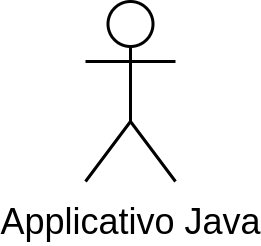
\includegraphics{capitolo3/casi-uso/attori-primari.png}
  \caption{Attori primari}
\end{figure}

\begin{itemize}
  \item \textbf{Applicativo Java}: rappresenta qualsiasi applicazione sviluppata in Java che interagisce con la libreria. In questo caso, consiste nel \textit{back-end} sviluppato utilizzando il \textit{framework} Spring.
\end{itemize}

\subsubsection{Attori secondari}
Un attore secondario è un'entità estranea al sistema che supporta gli attori primari nelle loro attività.

\begin{figure}[h!]
  \centering
  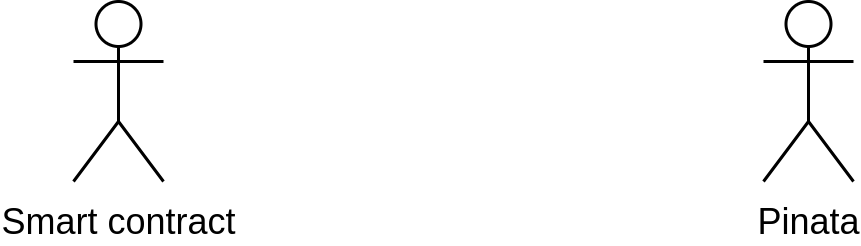
\includegraphics{capitolo3/casi-uso/attori-secondari.png}
  \caption{Attori secondari}
\end{figure}

\begin{itemize}
  \item \textbf{\textit{Smart contract}}: rappresenta lo \textit{smart contract} caricato in \textit{blockchain} con il quale comunicare;
  \item \textbf{Pinata}: rappresenta il servizio che permette di interagire con la rete IPFS.
\end{itemize}

\UC{Caricamento di un NFT in blockchain}
\label{UC:upload-new-nft}

Qualsiasi applicativo Java può caricare un nuovo NFT in blockchain.

\begin{itemize}
  \item \UCPrimaryActors{applicativo Java};
  \item \UCSecondaryActors{\textit{smart contract}, Pinata};
  \item \UCPre{l'applicativo Java vuole creare un NFT da un opera non ancora esistente};
  \item \UCPost{il NFT è stato creato e l'opera è stata caricata nella rete IPFS};
  \item \UCMain
  \begin{itemize}
    \item L'applicativo Java vuole creare un NFT a partire da un opera, dalla quale non è stato creato alcun NFT;
    \item L'opera viene caricata sulla rete IPFS tramite il servizio Pinata;
    \item Viene invocato lo \textit{smart contract} e creato il NFT.
  \end{itemize}
  \item \UCExt
  \begin{enumerate}[label=\lett]
    \item L'applicativo Java vuole assegnare il NFT ad un \textit{wallet} che non è nel formato corretto:
    \begin{itemize}
      \item (UC\ref{UC:extension.wallet-not-correct}) - Visualizzazione messaggio di \textit{wallet} non nel formato corretto;
      \item Viene impedita la creazione del NFT.
    \end{itemize}

    \item L'applicativo Java vuole comunicare con lo \textit{smart contract} attraverso un \textit{wallet}, il quale non è il proprietario di quest'ultimo:
    \begin{itemize}
      \item (UC\ref{UC:extension.operation-not-allowed}) - Visualizzazione messaggio di operazione non consentita;
      \item Viene impedita la creazione del NFT.
    \end{itemize}

    \item L'applicativo Java vuole caricare un'opera dalla quale è già stato estratto il NFT:
    \begin{itemize}
      \item (UC\ref{UC:extension.nft-exists-yet}) - Visualizzazione messaggio di NFT già esistente;
      \item Viene impedita la creazione del NFT.
    \end{itemize}
  \end{enumerate}
\end{itemize}


\UC{Trasferimento della proprietà di un NFT}
\label{UC:transfer-nft}

L'applicativo Java può trasferire la proprietà di un NFT dal proprietario ad un acquirente.

\begin{itemize}
  \item \UCPrimaryActors{applicativo Java};
  \item \UCSecondaryActors{\textit{smart contract}};
  \item \UCPre{esiste il NFT che si vuole trasferire e l'acquirente è diverso dal proprietario};
  \item \UCPost{il NFT viene trasferito dal proprietario all'acquirente};
  
  \item \UCMain
  \begin{itemize}
    \item L'applicativo Java, attraverso il \textit{wallet} del proprietario dello \textit{smart contract}, comunica con lo \textit{smart contract} caricato nella \textit{blockchain};
    \item Gli invia i dati del proprietario e dell'acquirente;
    \item Viene eseguito il trasferimento.
  \end{itemize}

  \item \UCExt
  \begin{enumerate}[label=\lett]
    \item L'applicativo Java vuole vuole trasferire il NFT dal proprietario all'acquirente, riferendosi ad uno di questi due attraverso un \textit{wallet} che non è nel formato corretto:
    \begin{itemize}
      \item (UC\ref{UC:extension.wallet-not-correct}) - Visualizzazione messaggio di \textit{wallet} non nel formato corretto;
      \item Viene impedito il trasferimento del NFT.
    \end{itemize}

    \item L'applicativo Java vuole comunicare con lo \textit{smart contract} attraverso un \textit{wallet}, il quale non è il proprietario di quest'ultimo:
    \begin{itemize}
      \item (UC\ref{UC:extension.operation-not-allowed}) - Visualizzazione messaggio di operazione non consentita;
      \item Viene impedito il trasferimento del NFT.
    \end{itemize}

    \item L'acquirente corrisponde al proprietario del NFT:
    \begin{itemize}
      \item Visualizzazione messaggio di operazione non andata a buon fine, dato che l'acquirente non può anche essere il proprietario del NFT;
      \item Viene impedito il trasferimento del NFT.
    \end{itemize}
  \end{enumerate}
\end{itemize}

\UC{Ottenimento di un NFT a partire dal suo id}
\label{UC:get-nft-by-id}

L'applicativo Java può ottenere le informazioni di un NFT a partire dal id con il quale è memorizzato.

\begin{itemize}
  \item \UCPrimaryActors{applicativo Java};
  \item \UCSecondaryActors{\textit{smart contract}};
  \item \UCPre{l'applicativo Java utilizza un id associato ad un NFT};
  \item \UCPost{l'applicativo Java ottiene le informazioni del NFT};
  \item \UCMain
  \begin{itemize}
    \item l'applicativo Java invoca lo \textit{smart contract} utilizzando un id associato ad un NFT;
    \item riceve le informazioni inserite durante la creazione.
  \end{itemize}

  \item \UCExt
  \begin{enumerate}[label=\lett]
    \item L'applicativo Java invia un id che non è associato ad alcun NFT:
    \begin{itemize}
      \item (UC\ref{UC:extension.nft-not-exists}) - Visualizzazione messaggio di NFT non esistente;
    \end{itemize}
  \end{enumerate}
\end{itemize}

\UC{Ottenimento di un opera a partire dal suo hash}
\label{UC:get-nft-by-hash}

L'applicativo Java può ottenere le informazioni di un NFT a partire dal hash associato al NFT.

\begin{itemize}
  \item \UCPrimaryActors{applicativo Java};
  \item \UCSecondaryActors{\textit{smart contract}};
  \item \UCPre{l'applicativo Java utilizza un hash associato ad un NFT};
  \item \UCPost{l'applicativo Java ottiene le informazioni del NFT};
  
  \item \UCMain
  \begin{itemize}
    \item l'applicativo Java invoca lo \textit{smart contract} utilizzando il hash associato al NFT;
    \item riceve le informazioni inserite durante la creazione. 
  \end{itemize}
  
  \item \UCExt
  \begin{enumerate}[label=\lett]
    \item l'applicativo Java invia un hash che non è associato ad alcun NFT:
    \begin{itemize}
      \item (UC\ref{UC:extension.nft-not-exists}) - Visualizzazione messaggio di NFT non esistente.
    \end{itemize}
  \end{enumerate}
\end{itemize}

\UC{Ottenimento della storia delle transazioni di un NFT}
\label{UC:get-transaction-history}

L'applicativo Java può ottenere la storia delle transazioni di un NFT a partire dal id con il quale è memorizzato.

\begin{itemize}
  \item \UCPrimaryActors{applicativo Java};
  \item \UCSecondaryActors{\textit{smart contract}};
  \item \UCPre{l'applicativo Java utilizza un id associato ad un NFT};
  \item \UCPost{L'applicativo Java ottiene la storia delle transazioni di un NFT};

  \item \UCMain
  \begin{itemize}
    \item l'applicativo Java invoca lo \textit{smart contract} utilizzando un id associato ad un NFT;
    \item riceve la storia delle transazioni.
  \end{itemize}
  
  \item \UCExt
  \begin{enumerate}[label=\lett]
    \item L'applicativo Java invia un id che non è associato ad alcun NFT:
    \begin{itemize}
      \item (UC\ref{UC:extension.nft-not-exists}) - Visualizzazione messaggio di NFT non esistente;
    \end{itemize}
  \end{enumerate}
\end{itemize}

\UC{Visualizzazione messaggio di wallet non nel formato corretto}
\label{UC:extension.wallet-not-correct}

Nel caso in cui il \textit{wallet} inviato allo \textit{smart contract} non sia nel formato corretto, verrà visualizzato un messaggio di errore che lo segnala.

\begin{itemize}
  \item \UCPrimaryActors{applicativo Java};
  \item \UCSecondaryActors{\textit{smart contract}};
  \item \UCPre{il formato del \textit{wallet} non è nel formato corretto};
  \item \UCPost{viene visualizzato il messaggio che segnala l'errore};
  
  \item \UCMain
  \begin{itemize}
    \item l'applicativo Java invia un \textit{wallet} che non è nel formato corretto;
    \item viene visualizzato il messaggio che segnala l'errore.
  \end{itemize}
\end{itemize}

\UC{Visualizzazione messaggio di operazione non consentita}
\label{UC:extension.operation-not-allowed}

Nel caso in cui lo \textit{smart contract} non venga invocato dal suo proprietario, verrà visualizzato il messaggio di operazione non consentita.

\begin{itemize}
  \item \UCPrimaryActors{applicativo Java};
  \item \UCSecondaryActors{\textit{smart contract}};
  \item \UCPre{lo \textit{smart contract} non viene invocato dal suo proprietario};
  \item \UCPost{viene visualizzato il messaggio di operazione non consentita};
  
  \item \UCMain
  \begin{itemize}
    \item l'applicativo Java non viene invocato dal suo proprietario;
    \item viene visualizzato il messaggio di operazione non consentita. 
  \end{itemize}
\end{itemize}

\UC{Visualizzazione messaggio di NFT già esistente}
\label{UC:extension.nft-exists-yet}

Nel caso in cui si cerchi di caricare un NFT già esistente, verrà visualizzato un messaggio opportuno che lo segnalerà.

\begin{itemize}
  \item \UCPrimaryActors{applicativo Java};
  \item \UCSecondaryActors{\textit{smart contract}};
  \item \UCPre{l'applicativo Java carica un NFT già esistente};
  \item \UCPost{viene visualizzato un messaggio di errore che lo segnala};
  
  \item \UCMain
  \begin{itemize}
    \item l'applicativo Java carica un NFT già esistente;
    \item viene visualizzato il messaggio di NFT già esistente.
  \end{itemize}
\end{itemize}

\UC{Visualizzazione messaggio di NFT non esistente}
\label{UC:extension.nft-not-exists}

Nel caso in cui il NFT di cui si ha bisogno non esista, verrà visualizzato un messaggio opportuno che lo segnalerà.

\begin{itemize}
  \item \UCPrimaryActors{applicativo Java};
  \item \UCSecondaryActors{\textit{smart contract}};
  \item \UCPre{il NFT che si sta cercando non esiste};
  \item \UCPost{viene visualizzato un messaggio di errore che segnala la non esistenza del NFT};
  
  \item \UCMain
  \begin{itemize}
    \item l'applicativo Java ha bisogno di un NFT non esistente;
    \item viene visualizzato il messaggio di NFT non esistente.
  \end{itemize}
\end{itemize}

\subsection{Requisiti funzionali}
Tabella dei requisiti funzionali, con relativa spiegazione e fonte.

\begin{longtabu}{|X[0.8,c]|X[3,c]|X[0.5,c]|}
  % \renewcommand{\arraystretch}{1.3}

  \hline 

  \textbf{Codice requisito} & \textbf{Descrizione} & \textbf{Fonte} \\ 

  \hline

  \rfun{O}{} & L'applicativo Java può caricare un nuovo NFT. & UC\ref{UC:upload-new-nft} \\
  
  \hline

  \rfun{O}{} & L'applicativo Java può trasferire la proprietà di un NFT dal proprietario all'acquirente. & UC\ref{UC:transfer-nft} \\ 
  
  \hline

  \rfun{O}{} & L'applicativo Java può ottenere le informazioni di un NFT a partire dall'id con il quale è memorizzato. & UC\ref{UC:get-nft-by-id} \\ 
  
  \hline

  \rfun{O}{} & L'applicativo Java può ottenere le informazioni di un NFT a partire dal hash al quale è associato. & UC\ref{UC:get-nft-by-hash} \\ 
  
  \hline

  \rfun{O}{} & L'applicativo Java può ottenere la storia delle transazioni di un NFT. & UC\ref{UC:get-transaction-history} \\ 
  
  \hline

  \caption{Requisiti funzionali}
\end{longtabu}

\subsection{Requisiti di qualità}
Tabella dei requisiti di qualità, con relativa spiegazione e fonte.

\begin{longtabu}{|c l c|}

  \hline 

  Codice requisito & Descrizione & Fonte \\ 
  
  \hline

  \caption{Requisiti di qualità}
\end{longtabu}

\subsection{Requisiti di vincolo}
Tabella dei requisiti di vincolo, con relativa spiegazione e fonte.

\begin{longtabu}{|c|l|c|}

  \hline 

  Codice requisito & Descrizione & Fonte \\ 
  
  \hline

  \caption{Requisiti di vincolo}
\end{longtabu}
